% !TEX encoding = UTF-8 Unicode

Ny$\bar{a}$ya for iPad is not the first program  that processes expressions of propositional logic. 
Besides powerful SAT-solvers and automatic provers, which rarely can be used by beginners,
there are some software products, that can be used on a basic level of experience with propositional logic and Boolean expressions.  
Most of them provide a (short) introduction to propositional logic, but they seldom offer tutorials or exercises. 	

The following list presents some software products accessible
via website and apps available for iPad.

\section{Websites}

\begin{itemize}
\item 
\href{http://www.cs.wfu.edu/~burg/JavaPackages/indexswingnet.html}{\bf PLogic Applet} 
by S. Lukins, A. Levicki, and 
\href{http://www.cs.wfu.edu/~burg}{J. Burg} at the
\href{http://www.cs.wfu.edu}{Wake Forest University}, is a
tutorial program for propositional logic 
“that serves a double role as an educational tool and a research environment”\footnote {
\url{http://www.cs.wfu.edu/~burg/papers/PropLogic.pdf}} and focuses 
 on interactive theorem-proving.

\item
\href{http://cl-informatik.uibk.ac.at/software/booltool/}{\bf 

\includegraphics[width=0.8cm]{clshortlogo_new.pdf}BoolTool} 
by the 
\href{http://cl-informatik.uibk.ac.at/}{Computational Logic} 
research group at the 
\href{http://informatik.uibk.ac.at}{University of Innsbruck}
“is an interface to the program BoolTool which allows the manipulation and evaluation of boolean functions.”\footnote{
\url{http://cl-informatik.uibk.ac.at/software/booltool/?page=info}}. 
It computes truth tables and binary decision diagrams and checks for satisfiability and validity.

\item
\href{http://www.wolframalpha.com/input/?i=a+or+b+and+c}{\bf 

\includegraphics[width=0.8cm]{related/WolframAlpha.jpg} Wolfram Alpha} 
by 
\href{http://www.wolfram.com/}{Wolfram Research} – the makers of 
\href{http://www.wolfram.com/mathematica/}{Mathematica} – supports
propositional logic by calculating truth tables and minimal forms, 
but does not draw syntax trees or binary decision diagrams.
Instead it draws a logic circuit and a Venn diagram from the input. 
Additionaly it calculates the truth density
and the boolean operator number of the input formula. 

Wolfram Alpha does not calculate exactly for an arbitrary number of variables in propositional formulas.
For example no truth table, conjunctive normal form, no disjunctive normal form is calculated
for the input
%\href{http://www.wolframalpha.com/input/?i=a⊻b⊻c⊻d⊻e⊻f⊻g⊻h⊻i⊻j}{
\href{http://www.wolframalpha.com/input/?i=a+xor+b+xor+c+xor+d+xor+e+xor+f+xor+g+xor+h+xor+i+xor+j}{
$a\veebar b\veebar c\veebar d\veebar e\veebar f\veebar g\veebar h\veebar i\veebar j$.}
The truth density is only sampled and does not match the exact result 0.5.
\end{itemize}

\section{Apps for iPad}
 
The following apps for iPad or iPod touch address aspects of propositional logic.

\begin{itemize}

\item  \href{http://itunes.apple.com/at/app/constraints/id418722652?mt=8}{\bf 
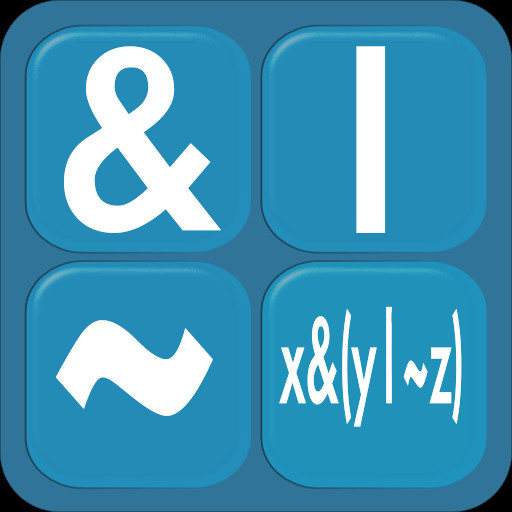
\includegraphics[width=0.8cm]{related/Constraints.png} Constraints}
by 
\href{http://www.mysvc.it/myapps/constraints/}{Davide Cucciniello} 
is a “SAT based propositional (boolean) logic engine defined by a list of models, 
where a model includes a list of constraints (a Knowledge Base) 
each defined by a propositional formula (x and (y or not z)) 
including a set of propositional (boolean) variables (x,y,z) 
and operators (and,or,not).”\footnote{
\url{http://www.mysvc.it/myapps/constraints/}} Constraints
lets you build models in an interactive way. 
It also provides a short introduction in propositional logic, 
but it does not provide any tutorials.


\item \href{http://itunes.apple.com/at/app/truth-table-generator/id507190346?mt=8}{\bf 
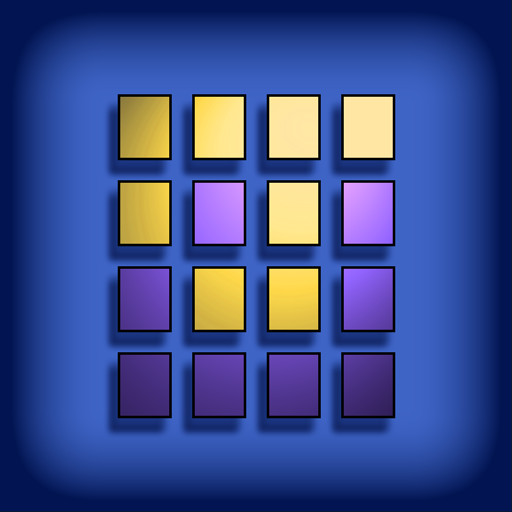
\includegraphics[width=0.8cm]{related/TruthTables.png} Truth Table Generator} 
by
\href{http://www.mertzwerkz.com/truth.html}{Mertz Werkz LLP}    
“constructs truth tables for the Boolean expressions you enter”.\footnote{
\url{http://www.mertzwerkz.com/truth.html}}
It does that nicely by using standard symbols of propositional logic (and a limited set of atoms), but nothing more.

\item
\href{http://itunes.apple.com/at/app/boolean-logic-cheat-sheet/id341959531?mt=8}{\bf 
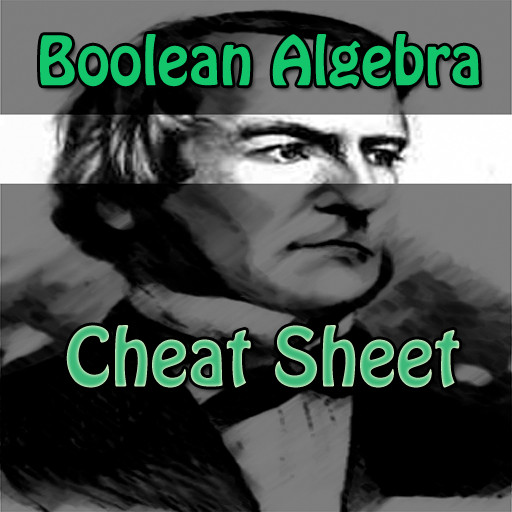
\includegraphics[width=0.8cm]{related/CheatSheet.png} Boolean Algebra Cheat Sheet} 
by 
{Clint Johnson} presents two pages of logic “rules and laws“ in low picture quality. So “Containing all of your Boolean 
logic needs.”\footnote{
\url{http://itunes.apple.com/at/app/boolean-logic-cheat-sheet/id341959531?mt=8}} 
does not feel quite right.

\item
\href{http://itunes.apple.com/at/app/logic-mania/id434019152?mt=8}{\bf 

\includegraphics[width=0.8cm]{related/LogicMania.png} Logic Mania} 
by 
{Imagination Creations} presents seven logic gates in a list. 
Their semantics are shown in a per-gate-simulation where the user chooses the input and the app shows the result. 
A combination of gates is not possible. It's quite nice but the statement “THE [sic] reference application for students 
studying logic gates”\footnote{
\url{http://itunes.apple.com/at/app/logic-mania/id434019152?mt=8}}
seems exaggerated.

\item
\href{http://itunes.apple.com/at/app/circuit-coder/id492180472?mt=8}{\bf 

\includegraphics[width=0.8cm]{related/CircuitCoder.png} Circuit Coder} 
by 
\href{http://sweyla.com/}{Trycycle Design HB} is a game about building digital circuits,
which is an application of propositional logic.

\end{itemize}
